\begin{figure*}[h]
\centering
\includegraphics[width=1.0\linewidth]{images/vis-comp-new-v1-crop.pdf}
\vspace{-20px}
\caption{Visualization comparison of robot motion generation for interactive sequences. We take two interaction cases as examples: "Link arms" (left) and "Wave" (right). Our method ("Ours") is shown alongside several baseline methods (JRT, MRT, ReGenNet, SAST) and the Ground Truth (GT). This visualization highlights that our model produces robot motions that are more natural, coherent, and closely aligned with the ground truth.}
%, particularly in terms of interaction smoothness, contact precision, and overall human-likeness, when compared to the other approaches.}
\label{fig:visintermodel-comp}
\vspace{-5px}
\end{figure*}

\begin{figure*}[b]
\centering
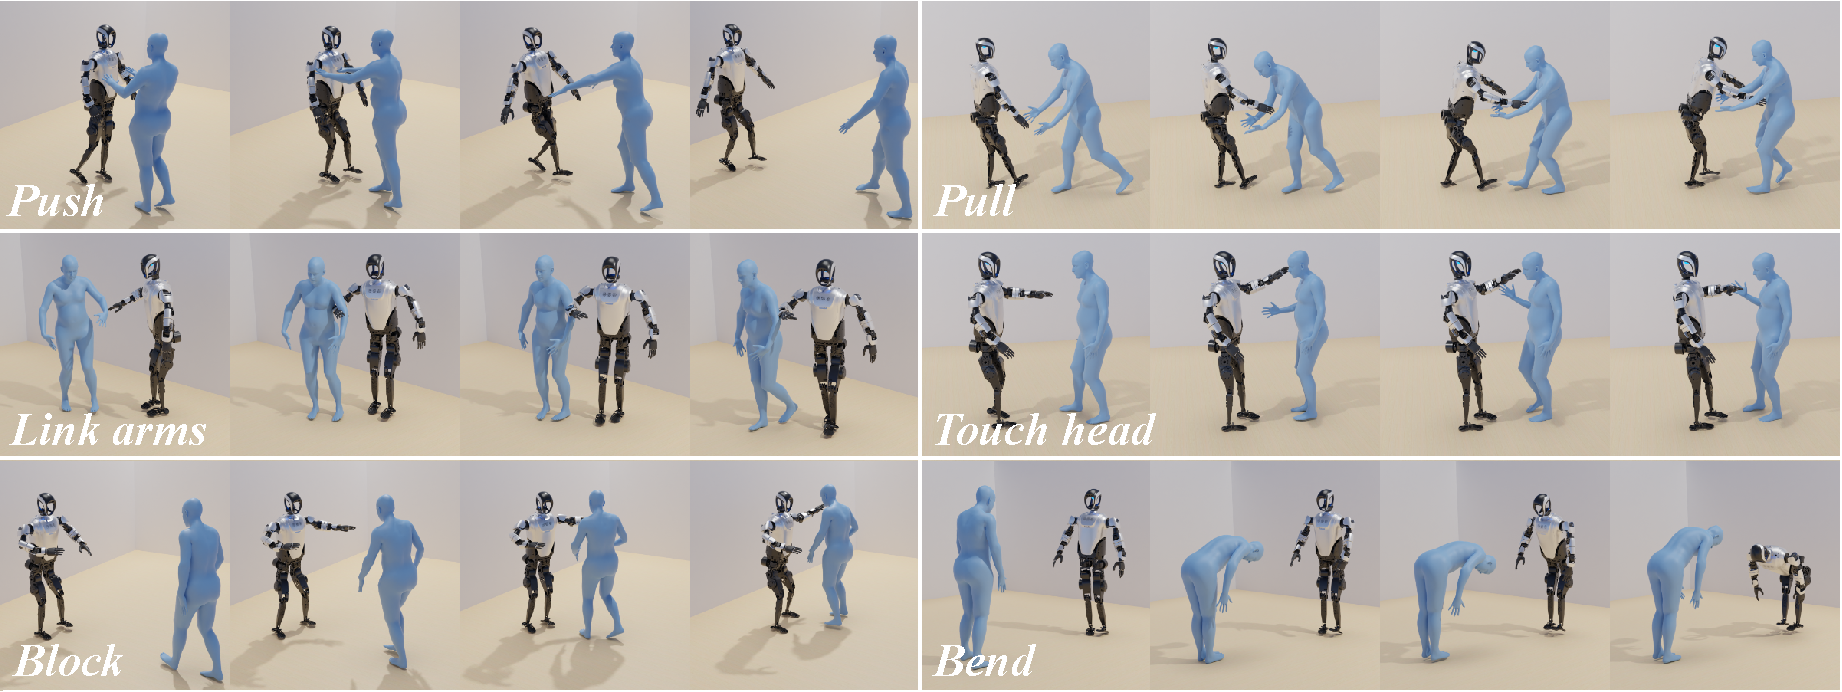
\includegraphics[width=1.0\linewidth]{images/vis-ours-new-1-v1-crop.pdf}
\end{figure*}
\begin{figure*}[h]
\centering
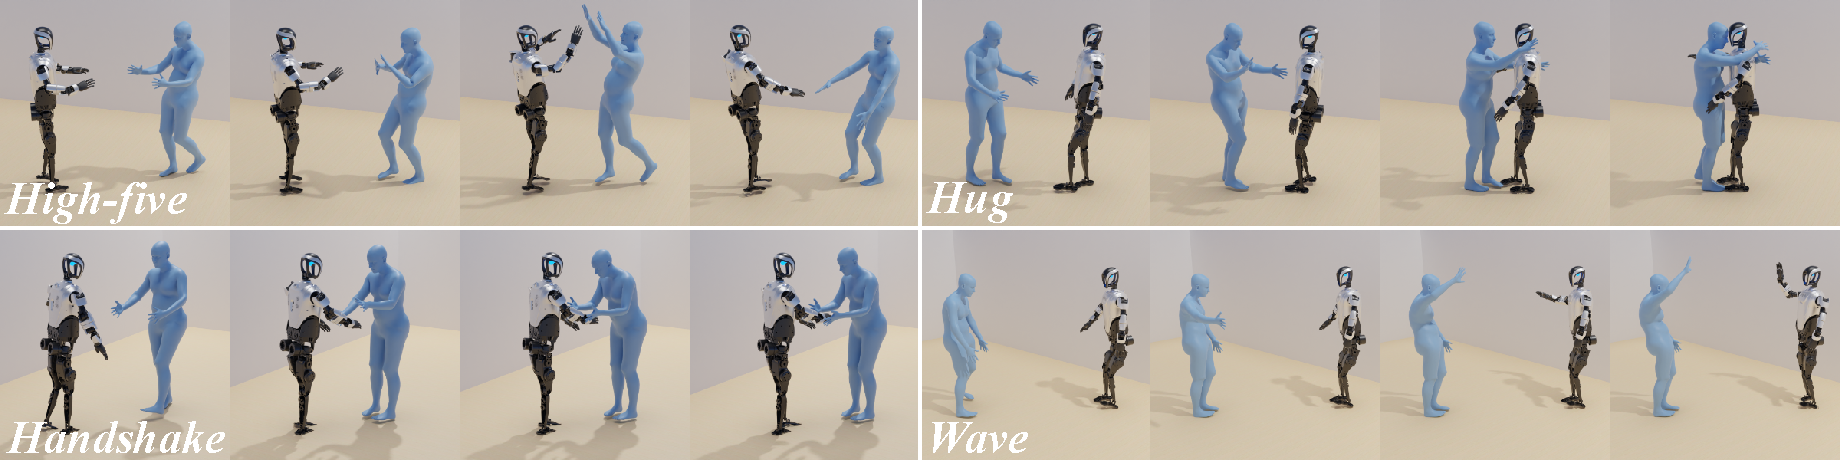
\includegraphics[width=1.0\linewidth]{images/vis-ours-new-0-v1-crop.pdf}
\vspace{-20px}
\caption{Visualizations of diverse human-robot interactions generated by our proposed Robotic Interaction Model. These sequences illustrate the model's capability to produce contextually appropriate and varied robot responses to dynamic human actions.}%, showcasing its effectiveness for enabling natural and engaging interactions.}%
\label{fig:visintermodel-ours}
\vspace{-5px}
\end{figure*}

